% -------------------------------------------------------------------------
% Setup
% -------------------------------------------------------------------------
\documentclass[11pt, aspectratio=149]{beamer}
% Options for aspectratio: 1610, 149, 54, 43 and 32, 169
\usepackage[utf8]{inputenc}
\usepackage[english]{babel}% Alternative: 'norsk'
\usepackage[expansion=false]{microtype}% Fixes to make typography better
\usecolortheme{beaver} % Decent options: beaver, rose, crane
\usepackage{listings}% To include source-code
\usepackage{booktabs}% Professional tables
\usefonttheme{serif}
\usepackage{mathptmx}
\usepackage[scaled=0.9]{helvet}
\usepackage{courier}

\title{Strength training programming}
\subtitle{Theory and practice}
\date{\today}
\author{Tommy (\texttt{tommyod @ github})}

% -------------------------------------------------------------------------
% Package imports
% -------------------------------------------------------------------------
\usepackage{etoolbox}
\usepackage{graphicx}
\usepackage{tikz}
\usepackage{amsmath}
\usepackage{amsthm}
\usepackage{amsfonts}
\usepackage{amssymb}
\usepackage{mathtools}
\usepackage{graphicx}
\usepackage{hyperref}
\usepackage{listings}
\usepackage[sharp]{easylist}
\usepackage{multicol}
\usepackage{tikz-cd}

% https://tex.stackexchange.com/questions/159667/including-python-code-in-beamer
% https://ftp.eq.uc.pt/software/TeX/macros/latex/contrib/minted/minted.pdf
\usepackage{minted}

\usefonttheme{professionalfonts}
\usepackage{fontspec}
\setmainfont{Open Sans}
\setsansfont{Open Sans}
\setmonofont{Ubuntu Mono}
\usefonttheme{serif}

%gets rid of bottom navigation bars
\setbeamertemplate{footline}[frame number]{}

%gets rid of bottom navigation symbols
\setbeamertemplate{navigation symbols}{}

% Set up colors to be used
\definecolor{purered}{RGB}{31,119,180}
\definecolor{titlered}{RGB}{31,119,180}
\definecolor{bggray}{RGB}{242,242,242}
\definecolor{bggraydark}{RGB}{217,217,217}

% Change the default colors

\setbeamercolor*{title}{bg=bggray,fg=titlered}
\AtBeginEnvironment{theorem}{%
	\setbeamercolor{block title}{fg=titlered, bg=bggraydark}
	\setbeamercolor{block body}{fg=black,bg=bggray}
}
\AtBeginEnvironment{proof}{%
	\setbeamercolor{block title}{bg=bggraydark}
	\setbeamercolor{block body}{fg=black,bg=bggray}
}
\AtBeginEnvironment{example}{%
	\setbeamercolor{block title example}{bg=bggraydark}
	\setbeamercolor{block body example}{fg=black,bg=bggray}
}
\AtBeginEnvironment{definition}{%
	\setbeamercolor{block title}{bg=bggraydark}
	\setbeamercolor{block body}{fg=black,bg=bggray}
}

\setbeamercolor{block title example}{bg=bggraydark}
\setbeamercolor{block body example}{fg=black,bg=bggray}
\setbeamercolor{block title}{bg=bggraydark}
\setbeamercolor{block body}{fg=black,bg=bggray}

\setbeamercolor{frametitle}{fg=titlered,bg=bggray}
\setbeamercolor{section in head/foot}{bg=black}
\setbeamercolor{author in head/foot}{bg=black}
\setbeamercolor{date in head/foot}{fg=titlered}


% Spacing for lsits
\newcommand{\listSpace}{0.4em}

% Theorems, equations, definitions setup
\theoremstyle{plain}

\usepackage{etoolbox}
\usepackage{lipsum}

\makeatletter
\patchcmd{\beamer@sectionintoc}
{\vfill}
{\vskip\itemsep}
{}
{}
\makeatother  

\AtBeginSection[]{
	\begin{frame}
		\vfill
		\centering
		\begin{beamercolorbox}[sep=8pt,center,shadow=false,rounded=false]{title}
			\usebeamerfont{title}\insertsectionhead\par%
		\end{beamercolorbox}
		\vfill
	\end{frame}
}

% -------------------------------------------------------------------------
% Document start
% -------------------------------------------------------------------------
\begin{document}
\maketitle

\begin{frame}[fragile, t]{Introduction}
\begin{columns}
\begin{column}{0.6\textwidth}
\textbf{This presentation}
\begin{easylist}[itemize]
	\ListProperties(Space=\listSpace, Space*=\listSpace)
	# Long term progress
	# Volume and intensity
	# Repetition schemes
	# \texttt{streprogen} Python package
\end{easylist}
\vspace*{2em}
\textbf{About me}
\begin{easylist}[itemize]
	\ListProperties(Space=\listSpace, Space*=\listSpace)
	# Training since 2005
	# Modeling since 1013
\end{easylist}
\end{column}
\begin{column}{0.4\textwidth}
	\begin{figure}
	\centering
	\includegraphics[width=0.99\linewidth]{tommy3_cropped_b.jpg}
\end{figure}
\end{column}
\end{columns}
\end{frame}

\section{Long term strength progression}

\begin{frame}[fragile, t]{The law of diminishing returns}
	\vfill
	Solve the differential equation $d S(t) / dt = k \left ( \text{GP} - S(t) \right )$.
	\vfill
	\begin{figure}
		\centering
		\includegraphics[width=\linewidth]{strength_progression_longterm.pdf}
	\end{figure}
	\vfill
\end{frame}

\begin{frame}[fragile, t]{Boundary correction}
	\vfill
	\begin{equation*}
		S( t) = (S_{i}-S_{f})e^{\alpha(t)k} + S_{f} + \alpha(t) (S_{i}-S_{f})e^{-k}, \quad \alpha(t) = \frac{ t_{i}-t }{t_{f}-t_{i}}
	\end{equation*}
	\vfill
	\begin{figure}
		\centering
		\includegraphics[width=\linewidth]{strength_progression_program_specific.pdf}
	\end{figure}
	\vfill
\end{frame}


\begin{frame}[fragile, t]{Sawtooth periodization}
	\vfill
	\begin{equation*}
S'( t) = S( t) \times \operatorname{sawtooth}(t)
\end{equation*}
	\vfill
	\begin{figure}
		\centering
		\includegraphics[width=\linewidth]{strength_progression_program_sawtooth_varying_nonlinearity.pdf}
	\end{figure}
	\vfill
\end{frame}


\begin{frame}[fragile, t]{Changing the period}
	\vfill
	\begin{figure}
		\centering
		\includegraphics[width=\linewidth]{strength_progression_program_sawtooth_varying_period.pdf}
	\end{figure}
	\vfill
\end{frame}

\begin{frame}[fragile, t]{Changing the scale (amplitude)}
	\vfill
	\begin{figure}
		\centering
		\includegraphics[width=\linewidth]{strength_progression_program_sawtooth_varying_scale.pdf}
	\end{figure}
	\vfill
\end{frame}

\begin{frame}[fragile, t]{Long term planning}
	\vfill
	\begin{figure}
		\centering
		\includegraphics[width=\linewidth]{strength_progression_sawtooth_longterm.pdf}
	\end{figure}
	\vfill
\end{frame}


\begin{frame}[fragile, t]{Sinusoidal periodization}
	\vfill
	\begin{figure}
		\centering
		\includegraphics[width=\linewidth]{strength_progression_program_sinusoidal_varying_period.pdf}
	\end{figure}
	\vfill
\end{frame}

\section{Repetitions and intensity}


\begin{frame}[fragile, t]{A typical relationship between repetitions and intensity}
	\vfill
	The function $I(r)$ takes a repetition $r$ and returns an intensity.
	\vfill
	\begin{figure}
		\centering
		\includegraphics[width=\linewidth]{reps_intensity_mapping.pdf}
	\end{figure}
	\vfill
\end{frame}


\begin{frame}[fragile, t]{Varying the relationship}
	\vfill
	If John has 120kg as his 1RM, 5 reps with the normal relationship means 120kg $\times \, I(5)$  $=$ 120kg $\times$ 0.868 $=$ 104.16kg $\approx$ 105kg.
	\vfill
	\begin{figure}
		\centering
		\includegraphics[width=\linewidth]{reps_intensity_mapping_many.pdf}
	\end{figure}
	\vfill
\end{frame}

\section{Volume and intensity}

\begin{frame}[fragile, t]{Typical program}
	\vspace*{-2em}
	\begin{align*}
		\text{Volume} &= \text{total reps} &&= \sum_{r_i \in s} r_i \\
		\text{Intensity} &= \text{avg intensity across sets} &&= \sum_{r_i \in s} r_i \times I(r_i) / \sum_{r_i \in s} r_i 
	\end{align*}
	\vspace*{-1em}
	\begin{figure}
		\centering
		\includegraphics[width=\linewidth]{periodization_reps_intensity.pdf}
	\end{figure}
	\vfill
\end{frame}


\begin{frame}[fragile, t]{Two consecutive programs}
	\vfill
	\begin{figure}
		\centering
		\includegraphics[width=\linewidth]{periodization_reps_intensity_double.pdf}
	\end{figure}
	\vfill
\end{frame}

\begin{frame}[fragile, t]{Periodization with shorter periods}
	\vfill
	\begin{figure}
		\centering
		\includegraphics[width=\linewidth]{periodization_reps_intensity_out_of_phase.pdf}
	\end{figure}
	\vfill
\end{frame}


\section{Repetition schemes}


\begin{frame}[fragile, t]{Introductory example}
	\vfill
	If sets of $\{2, 3, 4, 5 \}$ reps are allowed, how can we create a scheme with $12$ reps in total?
	\vfill
There are 12 ways, and they are:
	\vfill
	\begin{align*}
	(2, 2, 2, 2, 2, 2) &&
	(4, 2, 2, 2, 2) \\
	(3, 3, 2, 2, 2) &&
	(5, 3, 2, 2) \\
	(4, 4, 2, 2) &&
	(4, 3, 3, 2) \\
	(5, 5, 2) &&
	(3, 3, 3, 3) \\
	(5, 4, 3) &&
	(4, 4, 4)
	\end{align*}
	\vfill
\end{frame}



\begin{frame}[fragile, t]{Larger example and two issues}
	\vfill
	If sets of $\{3, 4, 5, 6, 7, 8 \}$ reps are allowed, how can we create a scheme with $25$ reps in total?
	\vfill
	There are 45 ways, some of which are:
	\vfill
	\begin{align*}
(4, 3, 3, 3, 3, 3, 3, 3)  &&
(8, 5, 3, 3, 3, 3)  \\
\mathbf{(8, 8, 3, 3, 3)} &&
(7, 7, 5, 3, 3) \\
\mathbf{(7, 6, 5, 4, 3)} &&
(8, 8, 6, 3)  \\
(5, 4, 4, 4, 4, 4)  &&
(8, 8, 5, 4) \\
(5, 5, 5, 5, 5) &&
(7, 6, 6, 6) 
	\end{align*}
	\vfill
\end{frame}


\begin{frame}[fragile, t]{Constraining the possibilities}
	\vfill
	If sets of $\{3, 4, 5, 6, 7, 8 \}$ reps are allowed, how can we create a scheme with $25$ reps in total subject to the constraints:
\vfill
	\begin{easylist}[itemize]
	\ListProperties(Space=\listSpace, Space*=\listSpace)
	# Max difference in repetitions equal to $1$ for adjacent sets.
	# Max number of unique sets in the scheme equal to $3$.
	\end{easylist}
	\vfill
	\begin{align*}
(4, 3, 3, 3, 3, 3, 3, 3) \, [92.7] &&
(5, 4, 4, 3, 3, 3, 3)\, [90.9] \\
(4, 4, 4, 4, 3, 3, 3)\, [91.1] &&
(5, 5, 5, 4, 3, 3)\, [88.8] \\
(5, 5, 4, 4, 4, 3)\, [89.1] &&
(5, 4, 4, 4, 4, 4)\, [89.3] \\
(6, 6, 5, 4, 4) \,[86.3] &&
(6, 5, 5, 5, 4) \,[86.6] \\
(5, 5, 5, 5, 5) \,[86.8] &&
(7, 7, 6, 5) \,[82.7] \\
(7, 6, 6, 6)\, [82.9] &&
	\end{align*}
\end{frame}


\begin{frame}[fragile, t]{Repetition schemes as an optimization problem}
	\vfill
	If sets of $\{3, 4, 5, 6, 7, 8 \}$ reps are allowed, how close to $25$ reps and $85$ intensity can we get, subject to the constraints:
	\vfill
	\begin{easylist}[itemize]
		\ListProperties(Space=\listSpace, Space*=\listSpace)
		# Max difference in repetitions equal to $1$ for adjacent sets.
		# Max number of unique sets in the scheme equal to $3$.
	\end{easylist}
	\begin{align*}
	s^\star &=  \underset{s}{\operatorname{argmin}} \, \left( I(s) - 85\right)^2 + \left( R(s) - 25\right)^2 \\
	s^\star &= (6, 6, 5, 5, 4)
	\end{align*}
	$I(s^\star) = 85.9$ and $R(s^\star) = 26$.
	\vfill
	If we relax the hard constraints we find $s^\star = (8, 6, 4, 4, 3)$, which has $I(s^\star) = 85.0$ and $R(s^\star) = 25$.
\end{frame}


\begin{frame}[fragile, t]{A large combinatorial problem}
	\vfill
	If sets of $\{1, 2, 3, 4, 5, 6, 7, 8 \}$ reps are allowed, there are $13561$ repetition schemes with $\leq 50$ repetitions in total.
	\vfill
	If set set the max difference in repetitions equal to $1$ for adjacent sets, and max number of unique sets in the scheme equal to $3$, only $855$ remain.
	\vfill
	Good software finds the optimal repetition scheme in milliseconds.
	\vfill
\end{frame}


\section{\texttt{streprogen}}


\begin{frame}[fragile, t]{Introduction}
	\begin{columns}
		\begin{column}{0.6\textwidth}
		You define duration, days, exercises, weights, intensity, volume, etc.
		\vspace*{1em}
		
		\texttt{streprogen} loops through weeks, then days, then exercises and finds the optimal repetition scheme.
		
		\begin{figure}
			\centering
			\includegraphics[width=\linewidth]{periodization_reps_intensity.pdf}
		\end{figure}
	
		\end{column}
		\begin{column}{0.4\textwidth}
			\begin{figure}
				\centering
				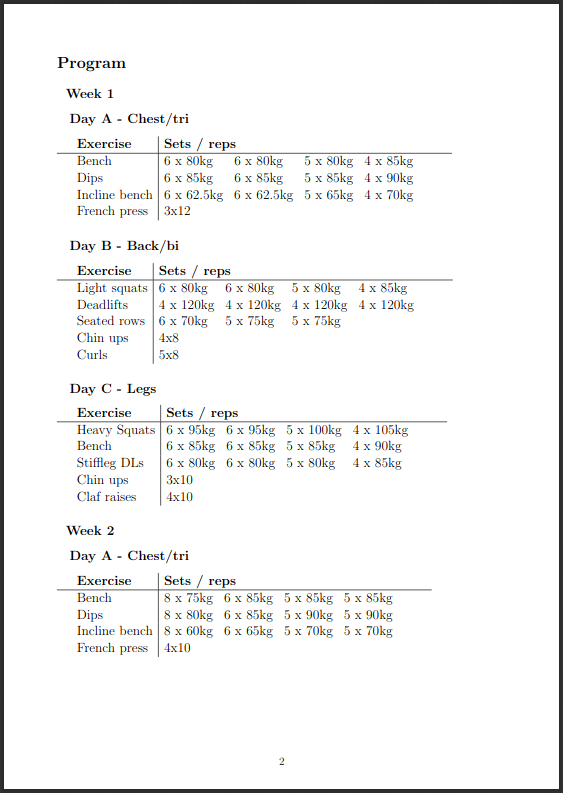
\includegraphics[width=1\linewidth]{streprogen_output.png}
			\end{figure}
		\end{column}
	\end{columns}
\end{frame}

\begin{frame}[fragile, t]{Defining a program}
\begin{minted}{python3}
from streprogen import Program

# Create an 8-week program
program = Program("My first program!", duration=8, round_to=5)

with program.Day("Day A"):
    program.DynamicExercise("Bench press", start_weight=80)
    program.DynamicExercise("Squats", start_weight=100)

with program.Day("Day B"):
    program.DynamicExercise("Deadlifts", start_weight=100)
    program.StaticExercise("Curls", "3 x 10 @ 18kg")

# Render the program, then print it
program.render()
print(program)
\end{minted}
\end{frame}

\begin{frame}[fragile, t]{Some program parameters}
\begin{minted}{python3}
program = Program(
    name='TommyAugust2020',
    duration=8,
    reps_per_exercise=25, 
    min_reps=3, 
    max_reps=8,
    percent_inc_per_week=1,
    intensity=85,
    rep_scaler_func=rep_scaler_func,
    intensity_scaler_func=intensity_scaler_func,
    units='kg',
    round_to=2.5,
)
\end{minted}
\end{frame}

\begin{frame}[fragile, t]{Some exercise parameters}
	\begin{minted}{python3}

program.DynamicExercise(name="Squats", start_weight=100)
    
program.DynamicExercise(name="Squats", 
                        start_weight=100, 
                        final_weight=120)
                                             
program.DynamicExercise(name="Squats", 
                        start_weight=100, 
                        percent_inc_per_week=2,
                        round_to=5,
                        reps=20,
                        max_reps=8, 
                        min_reps=5)
	\end{minted}
\end{frame}

\begin{frame}[fragile, t]{Summary}
	\vfill
	\textbf{Features in \texttt{streprogen}:}
	\begin{easylist}[itemize]
		\ListProperties(Space=\listSpace, Space*=\listSpace)
		# Any duration, any days per week, any volume, etc.
		# Many general functions for strength progression.
		# Combinatorial optimization for repetition schemes.
		# Simple and well-documented interface, easy to use.
		# Exports to text files, HTML or PDF.
	\end{easylist}
	\vfill
	\textbf{Further reading:}
\begin{easylist}[itemize]
	\ListProperties(Space=\listSpace, Space*=\listSpace)
	# GitHub: \texttt{https://github.com/tommyod/streprogen}
	# Issue tracker: \texttt{https://github.com/tommyod/streprogen/issues}
	# Theory: \texttt{https://tommyodland.com/}
	# Book: ``Practical Programming for Strength Training''
\end{easylist}
\vfill
\end{frame}





\end{document}
